\chapter{Report Generation}
\label{cha:reports}
\begin{quote}
If we spoke a different language, we would perceive a somewhat different world. --- Ludwig Wittgenstein
\end{quote}
\section{Overview}\label{sec:reports-overview}\index{report generation}
An overview of the report generation tools in \PyPedal{} is provided in this chapter.  The creation of a new, custom report is demonstrated.

\PyPedal{} has a framework in place to support basic report generation.  This franework consists of two components: a database access module, \module{pyp\_db} (Section \ref{sec:pyp-db}), and a reporting module, \module{pyp\_reports} (Section \ref{sec:pyp-reports}).  The SQLite 3 database engine (\url{http://www.sqlite.org/}) is used to store data and generate reports.  The ReportLab extension to Python (\url{http://www.reportlab.org/}) allows users to create reports in the Adobe Portable Document Format (PDF).  As a result, there are two types of reports that can be produced: internal summaries that can be fed to other \PyPedal{} routines (e.g. the report produced by \function{pyp\_reports.meanMetricBy()} can be passed to \function{pyp\_graphics.plot\_line\_xy()} to produce a plot) and printed reports in PDF format.  When referencing the \module{pyp\_reports} API note that the convention used in \PyPedal{} is that procedures which produce PDFs are prepended with 'pdf'.  Sections \ref{sec:reports-custom-internal-reports} and \ref{sec:reports-custom-printed-reports} demonstrate how to create new or custom reports.  \module{pyp\_reports} was added to \PyPedal{} with the intention that end-users develop their own custom reports using \function{pyp\_reports.meanMetricBy()} as a template.  More material on adding new functionality to \PyPedal{} can be found in Chapter \ref{cha:newfeatures}.

Column names, data types, and descriptions of contents for pedigree tables are presented in Table
\ref{tbl:reports-db-column-names}.  The \constant{metric\_to\_column} and \constant{byvar\_to\_column} dictionaries in
\module{pyp\_db} are used to convert between convenient mnemonics and database column names.  You may need to refer
to Table \ref{tbl:reports-db-column-names} for unmapped column names when writing custom reports.  If you happen
to view a table scheme using the \textbf{sqlite3} command-line utility you will notice that the columns are ordered
differently in the database than they are in the table; the table has been alphabetized for easy reference.
\begin{center}
    \tablecaption{Columns in pedigree database tables.}
    \tablefirsthead{\hline Name & Type & Note(s) \\ \hline}
    \tablehead{\hline Name & Type & Note(s) \\ \hline}
    \tabletail{\hline \multicolumn{3}{l}{\small\sl continued on next page} \\ \hline}
    \tablelasttail{\hline}
    \label{tbl:reports-db-column-names}
    \begin{xtabular}{llp{2.5in}}
	age           &   real          &  Age of animal \\
	alive         &   char(1)       &  Animal's mortality status \\
	ancestor      &   char(1)       &  Ancestor status \\
	animalID      &   integer       &  \textbf{Must be unique!} \\
	animalName    &   varchar(128)  &  Animal name \\
	birthyear     &   integer       &  Birth year \\
	breed         &   text          &  Breed \\
	coi           &   real          &  Coefficient of inbreeding \\
	damID         &   integer       &  Dam's ID \\
	founder       &   char(1)       &  Founder status \\
	gencoeff      &   real          &  Pattie's generation coefficient \\
	generation    &   real          &  Generation \\
	herd          &   integer       &  Herd ID \\
	infGeneration &   real          &  Inferred generation \\
	num\_daus     &   integer       &  Number of daughters \\
	num\_sons     &   integer       &  Number of sons \\
	num\_unk      &   integer       &  Offspring of unknown sex \\
	originalHerd  &   varchar(128)  &  Original herd ID \\
	originalID    &   text          &  Animal's original ID \\
	pedgreeComp   &   real          &  Pedigree completeness \\
	renumberedID  &   integer       &  Animal's renumbered ID \\
	sex           &   char(1)       &  Sex of animal \\
	sireID        &   integer       &  Sire's ID \\
    \end{xtabular}
\end{center}

\subsection{Three Generation Pedigrees}
\label{sec:reports-three-gen-peds}
\index{report generation!three generation pedigrees}
A report for producing three-generation pedigrees, \function{pdf3GenPed()}, is included in the \module{pyp_reports} module. The sample output shown in Figure \ref{fig:reports-three-gen-ped} contains output for one animal. However, if \function{pdf3GenPed()} is passed a list of animal IDs the resulting PDF will contain a pedigree for each animal that can be printed as a booklet. See Section \ref{sec:pyp-reports-pdf-three-gen-ped} for usage details.
\begin{figure}
  \begin{center}
    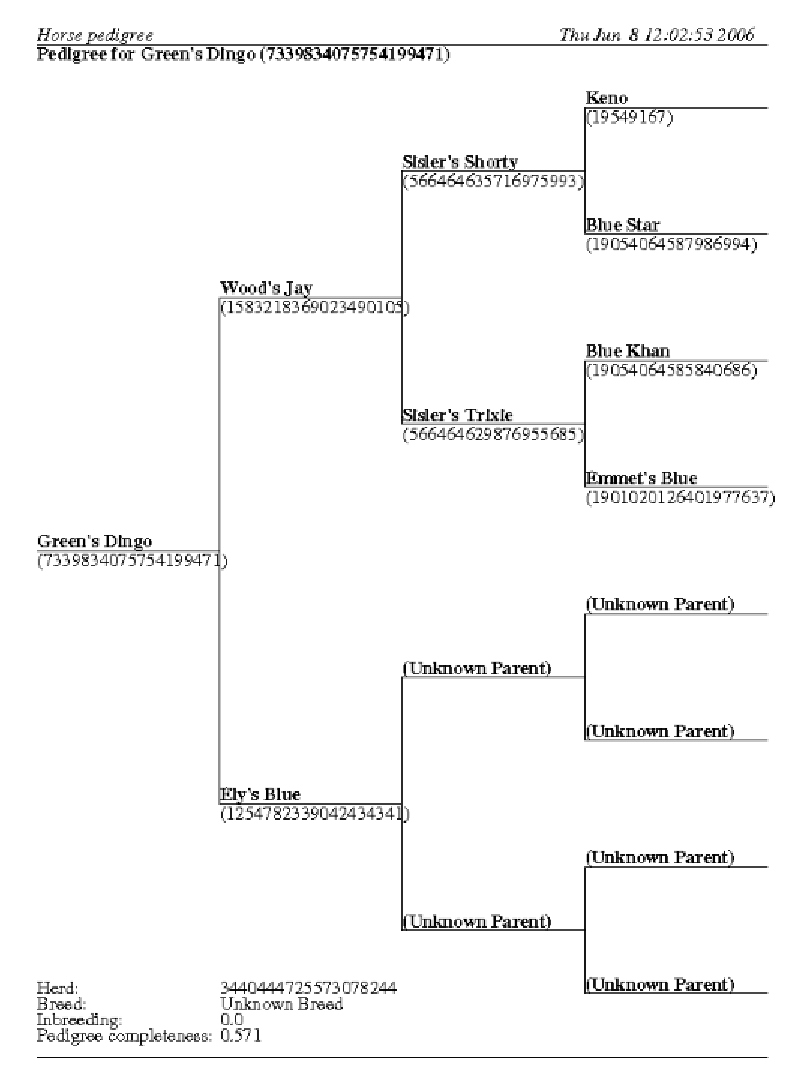
\includegraphics[width=6in]{greensDingoPedigree.eps}
    \caption{Example of a printed three generation pedigree.}
    \label{fig:reports-three-gen-ped}
  \end{center}
\end{figure}

\section{Creating a Custom Internal Report}
\label{sec:reports-custom-internal-reports}
\index{report generation!creating custom internal reports}
Internal reports \index{internal reports} typically aggregate data such that the result can be handed off to another \PyPedal{} routine for further processing.   To do this, the pedigree is loaded into a table in an SQLite database against which queries are made.  This is faster and more flexible than writing reporting routines that loop over the pedigree to construct reports, but it does require some knowledge of the Structured Query Language (SQL; \url{http://www.sql.org/}).  The canonical example of this kind of report is the passing of the dictionary returned by \function{pyp\_reports.meanMetricBy()} to \function{pyp\_graphics.plot\_line\_xy()} (see \ref{sec:graphics-drawing-pedigrees}).  That approach is outlined in code below.
\begin{verbatim}
def inbreedingByYear(pedobj):
    curs = pyp_db.getCursor(pedobj.kw['database_name'])

    # Check and see if the pedigree has already been loaded.  If not, do it.
    if not pyp_db.tableExists(pedobj.kw['database_name'], pedobj.kw['dbtable_name']):
        pyp_db.loadPedigreeTable(pedobj)

    MYQUERY = "SELECT birthyear, pyp_mean(coi) FROM %s GROUP BY birthyear \
        ORDER BY birthyear ASC" % (pedobj.kw['dbtable_name'])
    curs.execute(MYQUERY)
    myresult = curs.fetchall()
    result_dict = {}
    for _mr in myresult:
        _level, _mean = _mr
        result_dict[_level] = _mean
    return result_dict
\end{verbatim}
You should always check to see if your pedigree has been loaded into the database before you try and make queries against the pedigree table or your program may crash.  \function{inbreedingByYear()} returns a dictionary containing average coefficients of inbreeding keyed to birth years.  The query result, \var{myresult}, is a list of tuples; each tuple in the list
corresponds to one row in an SQL resultset. The tuples in \var{myresult} are unpacked into temporary variables that are then stored in the dictionary, \var{result\_dict} (for information on tuples see the Python Tutorial (\url{http://www.python.org/doc/tut/node7.html#SECTION007300000000000000000}).  If the resultset is empty, \var{result\_dict} will also be empty.  As long as you can write a valid SQL query for the report you'd like to assemble, there is no limitation on the reports that can be prepared by \PyPedal{}.
\section{Creating a Custom Printed Report}
\label{sec:reports-custom-printed-reports}
\index{report generation!creating custom printed reports}
If you are interested in custom printed reports you should begin by opening the file \texttt{pyp\_reports.py} and reading
through the code for the \function{pdfPedigreeMetadata()} report.  It has been heavily commented so that it can be used as
a template for developing other reports.  ReportLab provides fairly low-level tools that you can use to assemble
documents.  The basic idea is that you create a canvas on which your image will be drawn.  You then create text objects and
draw them on the canvas.  When your report is assembled you save the canvas on which it's drawn to a file.  \PyPedal{} provides
a few convenience functions for such commonly-used layouts as title pages and page "frames".  In the following sections of code I will discuss the creation of a \function{pdfInbreedingByYear()} printed report to accompany the
\function{inbreedingByYear()} internal report written in Section \ref{sec:reports-custom-internal-reports}.  First, we import ReportLab and check to see if the user provided an output file name.  If they didn't, revert to a default.
\begin{verbatim}
def pdfInbreedingByYear(pedobj,results,titlepage=0,reporttitle='',reportauthor='', \
    reportfile=''):
    import reportlab
    if reportfile == '':
        _pdfOutfile = '%s_inbreeding_by_year.pdf' % ( pedobj.kw['default_report'] )
    else:
        _pdfOutfile = reportfile
\end{verbatim}
Next call \function{\_pdfInitialize()}, which returns a dictionary of settings, mostly related to page size and
margin locations, that is used throughout the routine.  \function{\_pdfInitialize()} uses the \member{paper\_size} keyword
in the pedigree's options dictionary, which is either `letter' or `A4', and the \member{default\_unit}, which is either
`inch' or `cm' to populate the returned structure.  This should allow users to move between paper sizes without little
or no work.  Once the PDF settings have been computed we instantiate a canvas object on which to draw.
\begin{verbatim}
_pdfSettings = _pdfInitialize(pedobj)
canv = canvas.Canvas(_pdfOutfile, invariant=1)
canv.setPageCompression(1)
\end{verbatim}
There is a hook in the code to toggle cover pages on and off.  It is arguably rather pointless to put a cover page on a one-page document, but all TPS reports require new coversheets.  The call to \function{\_pdfDrawPageFrame()} frames the page with a header and footer that includes the pedigree name, date and time the report was created, and the page number.
\begin{verbatim}
if titlepage:
    if reporttitle == '':
        reporttitle = 'meanMetricBy Report for Pedigree\n%s' \
            % (pedobj.kw['pedname'])
    _pdfCreateTitlePage(canv, _pdfSettings, reporttitle, reportauthor)
_pdfDrawPageFrame(canv, _pdfSettings)
\end{verbatim}
The largest chunk of code in \function{pdfInbreedingByYear()} is dedicated to looping over the input dictionary, \var{results}, and writing its contents to text objects.  If you want to change the typeface for the rendered text, you need to make the appropriate changes to all calls to \texttt{canv.setFont("Times-Bold", 12)}.  The ReportLab documentation includes a discussion of available typefaces.
\begin{verbatim}
canv.setFont("Times-Bold", 12)
tx = canv.beginText( _pdfSettings['_pdfCalcs']['_left_margin'],
    _pdfSettings['_pdfCalcs']['_top_margin'] - 0.5 * \
        _pdfSettings['_pdfCalcs']['_unit'] )
\end{verbatim}
Every printed report will have a section of code in which the input is processed and written to text objects. In this case, the code loops over the key-and-value pairs in \var{results}, determines the width of the key, and creates a string with the proper spacing between the key and its value.  That string is then written to a \method{tx.textLine()} object.
\begin{verbatim}
# This is where the actual content is written to a text object that
# will be displayed on a canvas.
for _k, _v in results.iteritems():
    if len(str(_k)) <= 14:
        _line = '\t%s:\t\t%s' % (_k, _v)
    else:
        _line = '\t%s:\t%s' % (_k, _v)
    tx.textLine(_line)
\end{verbatim}
ReportLab's text objects do not automatically paginate themselves.  If you write, say, ten pages of material to a text object and render it without manually paginating the object you're going to get a single page of chopped-off text.  The following section of code is where the actual pagination occurs, so careful cutting-and-pasting should make pagination seamless.
\begin{verbatim}
    # Paginate the document if the contents of a textLine are longer than one page.
    if tx.getY() < _pdfSettings['_pdfCalcs']['_bottom_margin'] + \
        0.5 * _pdfSettings['_pdfCalcs']['_unit']:
        canv.drawText(tx)
        canv.showPage()
        _pdfDrawPageFrame(canv, _pdfSettings)
        canv.setFont('Times-Roman', 12)
        tx = canv.beginText( _pdfSettings['_pdfCalcs']['_left_margin'],
            _pdfSettings['_pdfCalcs']['_top_margin'] -
            0.5 * _pdfSettings['_pdfCalcs']['_unit'] )
\end{verbatim}
Once we're done writing our text to text objects we need to draw the text object on the canvas and make the canvas visible.  If you omit this step, perhaps because of the kind of horrible cutting-and-pasting accident to which I am prone, your PDF will not be written to a file.
\begin{verbatim}
if tx:
    canv.drawText(tx)
    canv.showPage()
canv.save()
\end{verbatim}
While \PyPedal{} does not yet have any standard reports that include graphics, ReportLab does support adding graphics, such as a pedigree drawing, to a canvas.  Interested readers should refer to the ReportLab documentation.